% !TeX root = ../main.tex
% Add the above to each chapter to make compiling the PDF easier in some editors.

\chapter{Evaluation}\label{chapter:evaluation}

This section aims to
evaluate how \ac{TRACER} performs at
modelling and synthesising user profiles
from a chatbot under testing.
To achieve this, the following research questions are addressed:

\begin{itemize}
\item \textbf{RQ1: How effective is TRACER in modelling chatbot functionality?}
  This question evaluates the capability of the proposed model discovery method to attain high functional coverage in a controlled environment where the ground truth is available.
\item \textbf{RQ2: How effective are the synthesised profiles at detecting faults in controlled environments?}
  This question tests the accuracy of the proposed method by applying mutation testing \autocite{gomez-abajoMutationTestingTaskOriented2024} to estimate the capacity of the created profiles to detect specific, injected faults.
\item \textbf{RQ3: How accurately does TRACER model the functionalities of real-world, deployed chatbots?}
  This question addresses the practical, real-world applicability of \ac{TRACER}.
  To answer it, we run \ac{TRACER} against a set of deployed chatbots,
  and then perform a manual verification of every functionality inferred.
  This allows us to measure the precision of the model,
  that is, the percentage of discovered functionalities that are correct and valid.
\end{itemize}

RQ1 evaluates the coverage of the proposed approach
in terms of activating chatbot functionalities.
To measure the coverage, \ac{TRACER} will be executed
against the chatbot under testing
and the generated synthesised profiles
will be executed with SENSEI against the same chatbot.
This process will be performed with chatbots created with the Taskyto framework
because this framework enables the reporting of the activated modules.
With these reports, it will be possible to measure
the coverage obtained during the \ac{TRACER} and SENSEI executions independently.

Higher coverage is anticipated during SENSEI profile execution,
as profiles are designed to systematically test all discovered parameters
and their valid combinations.
For instance, \ac{TRACER} may identify that a pizzeria chatbot
offers six pizza types, but does not try them all during exploration.
Instead, the generated profiles are designed to test all options.

Evaluating RQ1 is crucial for understanding
how thoroughly \ac{TRACER} exercises the chatbot’s functionality.
High coverage does not guarantee high quality,
but it implies that a significant part of a system has been tested,
increasing the confidence in its reliability
\autocite{ammannIntroductionSoftwareTesting2017}.


RQ2 assesses the practical effectiveness
of the proposed approach in detecting chatbot errors.
To this aim, mutation testing is employed
\autocite{demilloHintsTestData1978}
by introducing defects into correct chatbots to create mutants,
and testing whether the generated profiles detect these defects.
A profile successfully detects a mutation (i.e., a fault)
when the simulated user fails to complete a goal
(e.g., ordering a pizza type that was removed in the mutant)
or when an expected output is missing or incorrect.
Therefore, assessing RQ2 is important
for providing evidence that our approach produces
profiles that are sufficiently comprehensive
to reveal real-world chatbot errors.

RQ3 assesses \ac{TRACER}'s ability at modelling and synthesising
real-world deployed chatbots.
Unlike RQ1 and RQ2, which involves chatbots developed with the Taskyto framework
specifically for this evaluation,
RQ3 evaluates chatbots deployed for real-world applications
such as, universities, town halls or transportation companies.
To evaluate this, the model inferred by \ac{TRACER}
will be manually validated to measure the precision
of the discovered functionalities.

The experiment data is available at:
\url{https://github.com/Chatbot-TRACER/TRACER-evaluation}.

\section{RQ1: Coverage of Chatbot Functionality}

The primary goal of this first experiment
is to quantitatively measure the coverage
of \ac{TRACER} during its execution and
the subsequent execution of the generated user profiles with SENSEI.
To achieve this white-box evaluation
we ran the experiment in a controlled environment
using a chatbot whose source code is known,
which allowed us to measure the number of modules activated
during each conversation.

\subsection{Experiment Setup}

To assess the effectiveness of the proposed approach in discovering chatbot functionality,
we applied \ac{TRACER} to four deployed Taskyto chatbots
\autocite{sanchezcuadradoAutomatingDevelopmentTaskoriented2024}.
We chose chatbots built with this technology because their code is open-source
\autocite{SatorichatbotsTaskyto2025},
which allowed us to instrument them
to trace the modules activated during conversations,
as required to assess RQ1.
Moreover, the declarative structure of the chatbots
facilitated injecting faults into them, as required to assess RQ2.

Taskyto is a declarative framework
to develop LLM-based task-oriented chatbots using a YAML-like DSL.
Chatbot definitions consist of any number of modules of five possible types:

\begin{itemize}
  \item 
    \textbf{Menu:} to define conversation alternatives.
\item
  \textbf{Sequence:} to define a sequence of conversation steps.
\item
  \textbf{Action:} to execute Python code and produce a
verbatim or rephrased response upon receiving some input data.
\item
  \textbf{Data gathering:} to request user input data.
\item
  \textbf{Question answering:} to declare a FAQ.
\end{itemize}


\autoref{tab:rq1_chatbots} displays size metrics
of the chatbots used for this experiment.
We show the number of modules, lines of code (YAML lines),
input fields or parameters,
the number of possible values for these inputs in case that they are an enumeration,
and the number of question-answer pairs for the FAQ.

\textit{Bike-shop} schedules bike repair appointments
and answers bike maintenance questions.
\textit{Photography} is a chatbot for a photography shop,
which answers questions about the shop,
gathers contact details of clients, and provides price estimates.
\textit{Pizza-Order} handles pizza orders,
including their size, toppings and drinks.
\textit{Veterinary} sets appointments and answers questions about a veterinary clinic.

\begin{table}[htpb]
\centering
\caption{Size metrics of the four Taskyto chatbots used in the evaluation.}
\label{tab:rq1_chatbots}
\begin{tabular}{@{}lccccc@{}}
\toprule
\textbf{Chatbot} & \textbf{Modules} & \textbf{YAML lines} & \textbf{Inputs} & \textbf{Values} & \textbf{Q\&A Pairs} \\ \midrule
Bike-shop & 3 & 65 & 3 & 2 & 4 \\
Photography & 5 & 140 & 9 & 12 & 5 \\
Pizza-order & 10 & 282 & 22 & 78 & 6 \\
Veterinary & 3 & 71 & 3 & 4 & 5 \\ \bottomrule
\end{tabular}
\end{table}

We modified Taskyto to generate logs
for each conversation containing
each activated module,
expected input data from the user (e.g., pizza type),
values provided for the input data with a limited set of options (e.g., Carbonara),
and performed questions from the chatbot FAQ.
Subsequently, a Python script was used to unify these logs,
first by merging them into a unified log,
and then by generating a Markdown report
with the coverage percentage obtained for each chatbot.

To account for the non-deterministic nature of \acp{LLM},
we repeated the experiment three times.
To ensure that \ac{TRACER} finds as many functionalities as possible
we ran TRACER for 20 conversations with 12 turns each
to allow sufficient time for functionalities to branch out.
These parameters provide a balance between discovery and time.
The \ac{LLM} used by \ac{TRACER} was Google's Gemini 2.0 Flash
with the default model's parameters (1.0 temperature),
which we did not modify since it allowed creativity in the conversations
while still following \ac{TRACER}'s instructions.

SENSEI and Taskyto used OpenAI's GPT-4o-mini,
we used an OpenAI model
since these programs did not yet support a different provider
for Taskyto, the temperature was set to 0
to ensure the chatbot's behaviour was deterministic.
SENSEI used the temperatures defined in the generated profiles,
which as explained during the profile generation in \autoref{sec:profile-generation}
is set randomly.

The overall procedure then, is as follows.
First, we executed TRACER three times with the aforementioned settings
measuring the Taskyto coverage during each execution.
Using TRACER's generated profiles, we then ran SENSEI.
Since TRACER was run three times,
this resulted in three different sets of profiles.
Consequently, we measured the coverage for each of these three executions
and also reported an aggregated coverage.



\subsection{Results and Discussion}

\autoref{tab:rq1_coverage_results}
summarizes the results obtained throughout this experiment.
It contains the median and aggregated coverage obtained
during TRACER's exploration alone
and during the execution of the generated profiles within SENSEI.
The coverages are split into
modules, input parameters, values of these inputs and FAQ questions.
The table highlights in green the highest median and aggregate coverage
obtained per chatbot and metric
(i.e., module, input, value or question).

\begin{table}[!htb]
\centering
\caption{Coverage of TRACER (chatbot exploration) and SENSEI (profile execution).
In green there is the greatest coverage obtained
median and aggregate coverage per chatbot and metric
(i.e., module, input, value or question).
}
\label{tab:rq1_coverage_results}

% Define a custom color for the green highlight
\definecolor{lightgreen}{HTML}{C9FBC9}
\definecolor{stronggreen}{HTML}{53E753}

\begin{tabular}{lccccc}
\toprule
\textbf{Stat.} & \textbf{Tool} & \textbf{Module (\%)} & \textbf{Input (\%)} & \textbf{Value (\%)} & \textbf{Question (\%)} \\ \midrule

% --- Bike-shop Data ---
\rowcolor{gray!10} \multicolumn{6}{c}{\textbf{Bike-shop}} \\
\raisebox{-0.5\normalbaselineskip}[0pt][0pt]{Median} & TRACER & \cellcolor{lightgreen}100 & \cellcolor{stronggreen}85.71 & \cellcolor{stronggreen}83.33 & \cellcolor{stronggreen}75.00 \\
& SENSEI & \cellcolor{lightgreen}100 & 71.43 & 50.00 & 50.00 \\ \addlinespace
\raisebox{-0.5\normalbaselineskip}[0pt][0pt]{Aggregate} & TRACER & \cellcolor{lightgreen}100 & \cellcolor{lightgreen}85.71 & \cellcolor{lightgreen}83.33 & \cellcolor{stronggreen}75.00 \\
& SENSEI & \cellcolor{lightgreen}100 & \cellcolor{lightgreen}85.71 & \cellcolor{lightgreen}83.33 & 50.00 \\ \midrule

% --- Photography Data ---
\rowcolor{gray!10} \multicolumn{6}{c}{\textbf{Photography}} \\
\raisebox{-0.5\normalbaselineskip}[0pt][0pt]{Median} & TRACER & \cellcolor{lightgreen}100 & 73.33 & \cellcolor{stronggreen}64.71 & 20.00 \\
& SENSEI & \cellcolor{lightgreen}100 & \cellcolor{stronggreen}80.00 & 58.82 & \cellcolor{stronggreen}40.00 \\ \addlinespace
\raisebox{-0.5\normalbaselineskip}[0pt][0pt]{Aggregate} & TRACER & \cellcolor{lightgreen}100 & 73.33 & 76.47 & 20.00 \\
& SENSEI & \cellcolor{lightgreen}100 & \cellcolor{stronggreen}93.33 & \cellcolor{stronggreen}94.12 & \cellcolor{stronggreen}80.00 \\ \midrule

% --- Pizza-order Data ---
\rowcolor{gray!10} \multicolumn{6}{c}{\textbf{Pizza-order}} \\
\raisebox{-0.5\normalbaselineskip}[0pt][0pt]{Median} & TRACER & 83.33 & 67.86 & 27.38 & \cellcolor{lightgreen}100 \\
& SENSEI & \cellcolor{lightgreen}100 & \cellcolor{stronggreen}96.43 & \cellcolor{stronggreen}69.05 & \cellcolor{lightgreen}100 \\ \addlinespace
\raisebox{-0.5\normalbaselineskip}[0pt][0pt]{Aggregate} & TRACER & \cellcolor{lightgreen}100 & \cellcolor{lightgreen}100 & 48.81 & \cellcolor{lightgreen}100 \\
& SENSEI & \cellcolor{lightgreen}100 & \cellcolor{lightgreen}100 & \cellcolor{stronggreen}90.48 & \cellcolor{lightgreen}100 \\ \midrule

% --- Veterinary Data ---
\rowcolor{gray!10} \multicolumn{6}{c}{\textbf{Veterinary}} \\
\raisebox{-0.5\normalbaselineskip}[0pt][0pt]{Median} & TRACER & \cellcolor{lightgreen}100 & 50.00 & \cellcolor{lightgreen}44.44 & 20.00 \\
& SENSEI & \cellcolor{lightgreen}100 & \cellcolor{stronggreen}62.50 & \cellcolor{lightgreen}44.44 & \cellcolor{stronggreen}40.00 \\ \addlinespace
\raisebox{-0.5\normalbaselineskip}[0pt][0pt]{Aggregate} & TRACER & \cellcolor{lightgreen}100 & 62.50 & 55.56 & 40.00 \\
& SENSEI & \cellcolor{lightgreen}100 & \cellcolor{stronggreen}87.50 & \cellcolor{stronggreen}77.78 & \cellcolor{stronggreen}80.00 \\ \bottomrule
\end{tabular}
\end{table}

Regarding activated modules
both \ac{TRACER} and SENSEI achieved a 100\% aggregate coverage
across all chatbots,
and similarly for the median coverage, except for one case where
\ac{TRACER} achieved an 83.33\%.
This shows that the core functionalities of all chatbots
were successfully discovered during the exploration
and exercised during the profile execution.

In terms of the input parameters and
the values that these input fields allow,
we also obtained high values,
with a minimum value of 62.50\% aggregated value for TRACER
and a 85.71\% for SENSEI,
with both reaching a 100\% for the \textit{Pizza-order} chatbot.
For the values that these fields can take, we obtained
coverages as low as 48.81\% or 55.56\% in the aggregate \ac{TRACER} coverage,
but then for SENSEI we obtained higher values between 77.78\% and 94.12\%.
This was expected since during the exploration
TRACER might find values or options and not explore them further
but they are subsequently used in the profiles,
which means that SENSEI will use these values.
A clear example of this is the aggregate coverage in the \textit{pizza-order} values,
with only a 48.81\% during exploration but a 90.48\% for the profiles,
This example shows a greater jump since as shown in \autoref{tab:rq1_chatbots}
this chatbot has the highest number of values
(78 values, while the other chatbots have 2, 12 and 4).
This shows that the profile creation is comprehensive.

Lastly, aggregate question coverage was somewhat lower,
with SENSEI oscillating between a 50 and a 100\%.
This is the only metric where the aggregate coverage of TRACER
was higher than SENSEI's, which is contrary to the expected outcome.
This occurred because Taskyto sometimes struggles with FAQs;
if the question is not asked exactly as it is written,
Taskyto often fails to identify it.
\ac{TRACER} asked it as it was written in the FAQ
"Which is the price of a new tire?"
while SENSEI used "What is the price of a new tire?"
and Taskyto did not proceed with the answer, thus,
not adding it to the coverage logs.

\subsection{Answer to RQ1}

We conclude that \ac{TRACER} is able to effectively identify
most of a chatbot's functionalities, input parameters and values for these inputs.
Furthermore, we can conclude that TRACER effectively models the chatbot
since the inferred model used to generate the user profiles for SENSEI
managed to achieve aggregated coverages in the 77.78\% to the 100\% range
except for the outlier in the \textit{Bike-shop} FAQ.

\subsection{Threats to Validity}
The primary threat to this experiment
is related to external validity.
The evaluation was conducted exclusively
on four chatbots built with the Taskyto framework.
While this choice was necessary
to enable white-box coverage analysis,
it limits the generalisability of the findings.
The high coverage results
may not be representative of TRACER's performance
on chatbots built with different architectures,
such as intent-based systems like Rasa
or complex multi-agent frameworks.


\section{RQ2: Effectiveness in Detecting Faults}

After establishing \ac{TRACER}'s effectiveness at
discovering chatbot functionalities (RQ1),
this second experiment aims to assess
the practical fault detection capability
of the synthesised user profiles.
To this end, we will use mutation testing
\autocite{demilloHintsTestData1978}
to create faulty versions of the chatbots (mutants)
and measure the percentage of these faults
that are detected when executing the generated user profiles with SENSEI.

\subsection{Experiment Setup}

We applied mutations (i.e., injected errors)
to the four chatbots used in the previous RQ.
To choose the user profiles,
we selected the set that achieved the highest coverage
out of the three sets generated during RQ1.

To create the mutants we used a Python script
that generates as many mutant chatbots as possible from a given original,
introducing a single error in each mutant.
It achieves this by systematically injecting
single faults into the chatbot's YAML definition.
The following mutation operators are based on previous work
on mutation testing for task-oriented chatbots
\autocite{gomez-abajoMutationTestingTaskOriented2024, urricoMutaBotMutationTesting2024}:

\begin{itemize}
  \item \textbf{Delete Enum Value:}
    deleting a possible value from an input parameter
    (e.g., removing \texttt{small} from \texttt{pizza\_size}).
  \item \textbf{Change Optionality:}
    making an optional parameter required, or vice-versa.
  \item \textbf{Delete QA Pair:}
    removing a question from a FAQ module.
  \item \textbf{Swap QA Answer:}
    swapping the answers of two questions.
  \item \textbf{Delete Menu Alternative:}
    removing a conversational choice from a menu module.
  \item \textbf{Delete Fallback:}
    removing the fallback response.
  \item \textbf{Delete Sequence Step:}
    removing a necessary step from a workflow.
  \item \textbf{Swap Sequence Steps:}
    swapping the order of two steps in a sequence.
  \item \textbf{Delete Output Data:}
    omitting a piece of data from a chatbot's response (e.g., the price).
  \item \textbf{Change Rephrase Behavior:}
    altering the LLM's rephrasing mode.
  \item \textbf{Change Memory Scope:}
    changing the chatbot's ability to access data from previous turns.
\end{itemize}

The script systematically injects faults in every possible location of the chatbots.
However, due to the time and cost of running SENSEI,
we randomly selected two mutants of each type for each chatbot.
If only one or zero mutants of a type existed, all were selected.

A mutant is considered "killed"
if, during the execution of the SENSEI profiles,
at least one of the following conditions is met:
\begin{itemize}
  \item The simulation results in a crash, timeout, or conversation loop.
  \item A specified conversation \texttt{goal} is not achieved
    (e.g., the user fails to order the pizza).
  \item An expected \texttt{output} is missing or incorrect.
\end{itemize}


\subsection{Results and Discussion}

\begin{table}[htpb]
\centering
\caption{Summary of the mutation analysis results for each chatbot.}
\label{tab:rq2_mutation_results}
\begin{tabular}{@{}lcccccc@{}}
\toprule
\textbf{Chatbot} & \makecell[c]{\textbf{\# Mutants}} & \makecell[c]{\textbf{\# Profiles}} & \makecell[c]{\textbf{\# Convs.}\\\textbf{Per Chatbot}} & \makecell[c]{\textbf{Total}\\\textbf{Convs.}} & \makecell[c]{\textbf{Mutation}\\\textbf{Score (\%)}} & \makecell[c]{\textbf{\# Live}\\\textbf{Mutants}} \\ \midrule
Bike-shop & 13 & 3 & 9 & 117 & 91.0 & 1 \\
Photography & 18 & 3 & 12 & 216 & 76.9 & 3 \\
Pizza-order & 20 & 4 & 22 & 440 & 75.0 & 3 \\
Veterinary & 13 & 5 & 21 & 273 & 91.7 & 1 \\ \midrule
\textbf{TOTAL} & \textbf{64} & \textbf{15} & \textbf{64} & \textbf{1046} & \textbf{84.6} & \textbf{8} \\ \bottomrule
\end{tabular}
\end{table}

\autoref{tab:rq2_mutation_results}
shows the results for each chatbot.
The column \texttt{\# Mutants} represents
the total number of mutants generated
following the rule of selecting a maximum of 2 per mutation type.
\texttt{\# Profiles} shows the amount of profiles used
followed by \texttt{\# Convs. Per Chatbot},
which represents the total number of conversations
that occur by using the set of profiles from the previous column.
\texttt{Total Convs.} is the product of
\texttt{\# Mutants} and \texttt{\# Convs. Per Chatbot}
since each mutant is a new chatbot.
Finally, \texttt{Mutation Score (\%)} and \texttt{\# Live Mutants}
show the results from the executions.
\ac{MS} is the percentage of the mutants that were killed,
while the number of live mutants
represents the number of errors that were not found.

We observe a high overall \acl{MS}
with an average \ac{MS} of 84.6\%.
All chatbots achieved at least 75.0\%,
and peaking at 91.0\%.
The cases with the lowest \ac{MS}
(75.0\% and 76.9\%)
correspond to the most complex chatbots
(see \autoref{tab:rq1_chatbots}).

Although most of the errors were detected automatically (58\%),
some cases required manually inspecting the conversation,
e.g., when the chatbot omitted a specific piece of data
(such as the location of the photography shop)
but included other requested information.
For instance, the Photography chatbot outputs a summary of the shop information,
and some but not all information is set in this output,
therefore, there is no error of an unachieved goal,
even if the response is incomplete.
To detect such errors automatically,
detecting such errors automatically
would require testing rules that set oracles
and analyse the expected chatbot output values,
as explained in \autocite{delaraSensei}.

\subsection{Answer to RQ2}

The high mutation scores achieved (84.6\% on average)
provide strong evidence
that the profiles synthesised by TRACER are effective
at detecting faults in controlled environments.
However, full automation would require
complementing the profiles with (manually created) testing rules
that search for specific data in the profile outputs.



\section{RQ3: Accuracy of Modeling Deployed Chatbots}

The goal of RQ3 is to evaluate \ac{TRACER} in a realistic environment,
using a black-box chatbot for which the ground truth is unknown.
Unlike the controlled environments of RQ1 and RQ2,
this evaluation uses publicly deployed, real-world chatbots.
The goal is to measure the precision of \ac{TRACER}'s inferred model,
defined as the percentage of discovered functionalities that are correct and valid.
We chose this metric over others, such as recall,
because we do not have access to the complete model.
Therefore, we cannot determine
if the inferred model is missing any functionality.

\subsection{Experiment Setup}

For this experiment, we selected five different real-world deployed chatbots.
Ada-UAM \autocite{AdaUAM},
Gallo de Morón de la Frontera \autocite{AyuntamientoMoronFrontera},
Madrid te Cuida \autocite{ChatbotMadridTe},
Gestri (Diputación de Valencia) \autocite{DiputacionAtiendeMas},
and Ayuntamiento de Arucas \autocite{AyuntamientoArucasASISTENTES}.

Ada-UAM is a university support chatbot.
Gallo de Morón de la Frontera and Ayuntamiento de Arucas
are citizen services chatbots for town halls.
Gestri offers a chatbot that assists with the payment of taxes.
Lastly, Madrid te Cuida offers sanitary assistance.

These chatbots were chosen because they represent
genuine production systems from various public sector domains.
All of them were easily accessible through an \ac{API}.

The first stage of the protocol was to execute \ac{TRACER}
against each of these five chatbots.
To maintain consistency with the previous research questions,
we ran \ac{TRACER} with 20 sessions, each with 12 turns,
and chose Gemini 2.0 Flash as the \ac{LLM}.

The second stage was the manual verification.
The verification was performed for each functionality
and it involved interacting with the chatbot
and validating that the chatbot exhibits that functionality.
We also checked for duplicate functionalities.
Based on this verification,
each of TRACER's discovered functionalities was classified
as either a \ac{TP} or a \ac{FP}.
With the results, we computed the precision
(see \autoref{eq:precision}),
a metric that measures the correctness and accuracy of
\ac{TRACER}'s output.

\begin{equation}
\label{eq:precision}
\text{Precision} = \frac{\mathrm{TP}}{\mathrm{TP} + \mathrm{FP}}
\end{equation}

\begin{itemize}
  \item \textbf{\acf{TP}:}
    The number of functionalities discovered by \ac{TRACER}
    that were confirmed to be real, valid, and distinct.
  \item \textbf{\acf{FP}:}
    The number of functionalities discovered by \ac{TRACER}
    that were either incorrect
    (not actually present in the chatbot)
    or were duplicates of another functionality.
\end{itemize}

\subsection{Results and Discussion}

\begin{figure}[!htb]
  \begin{center}
    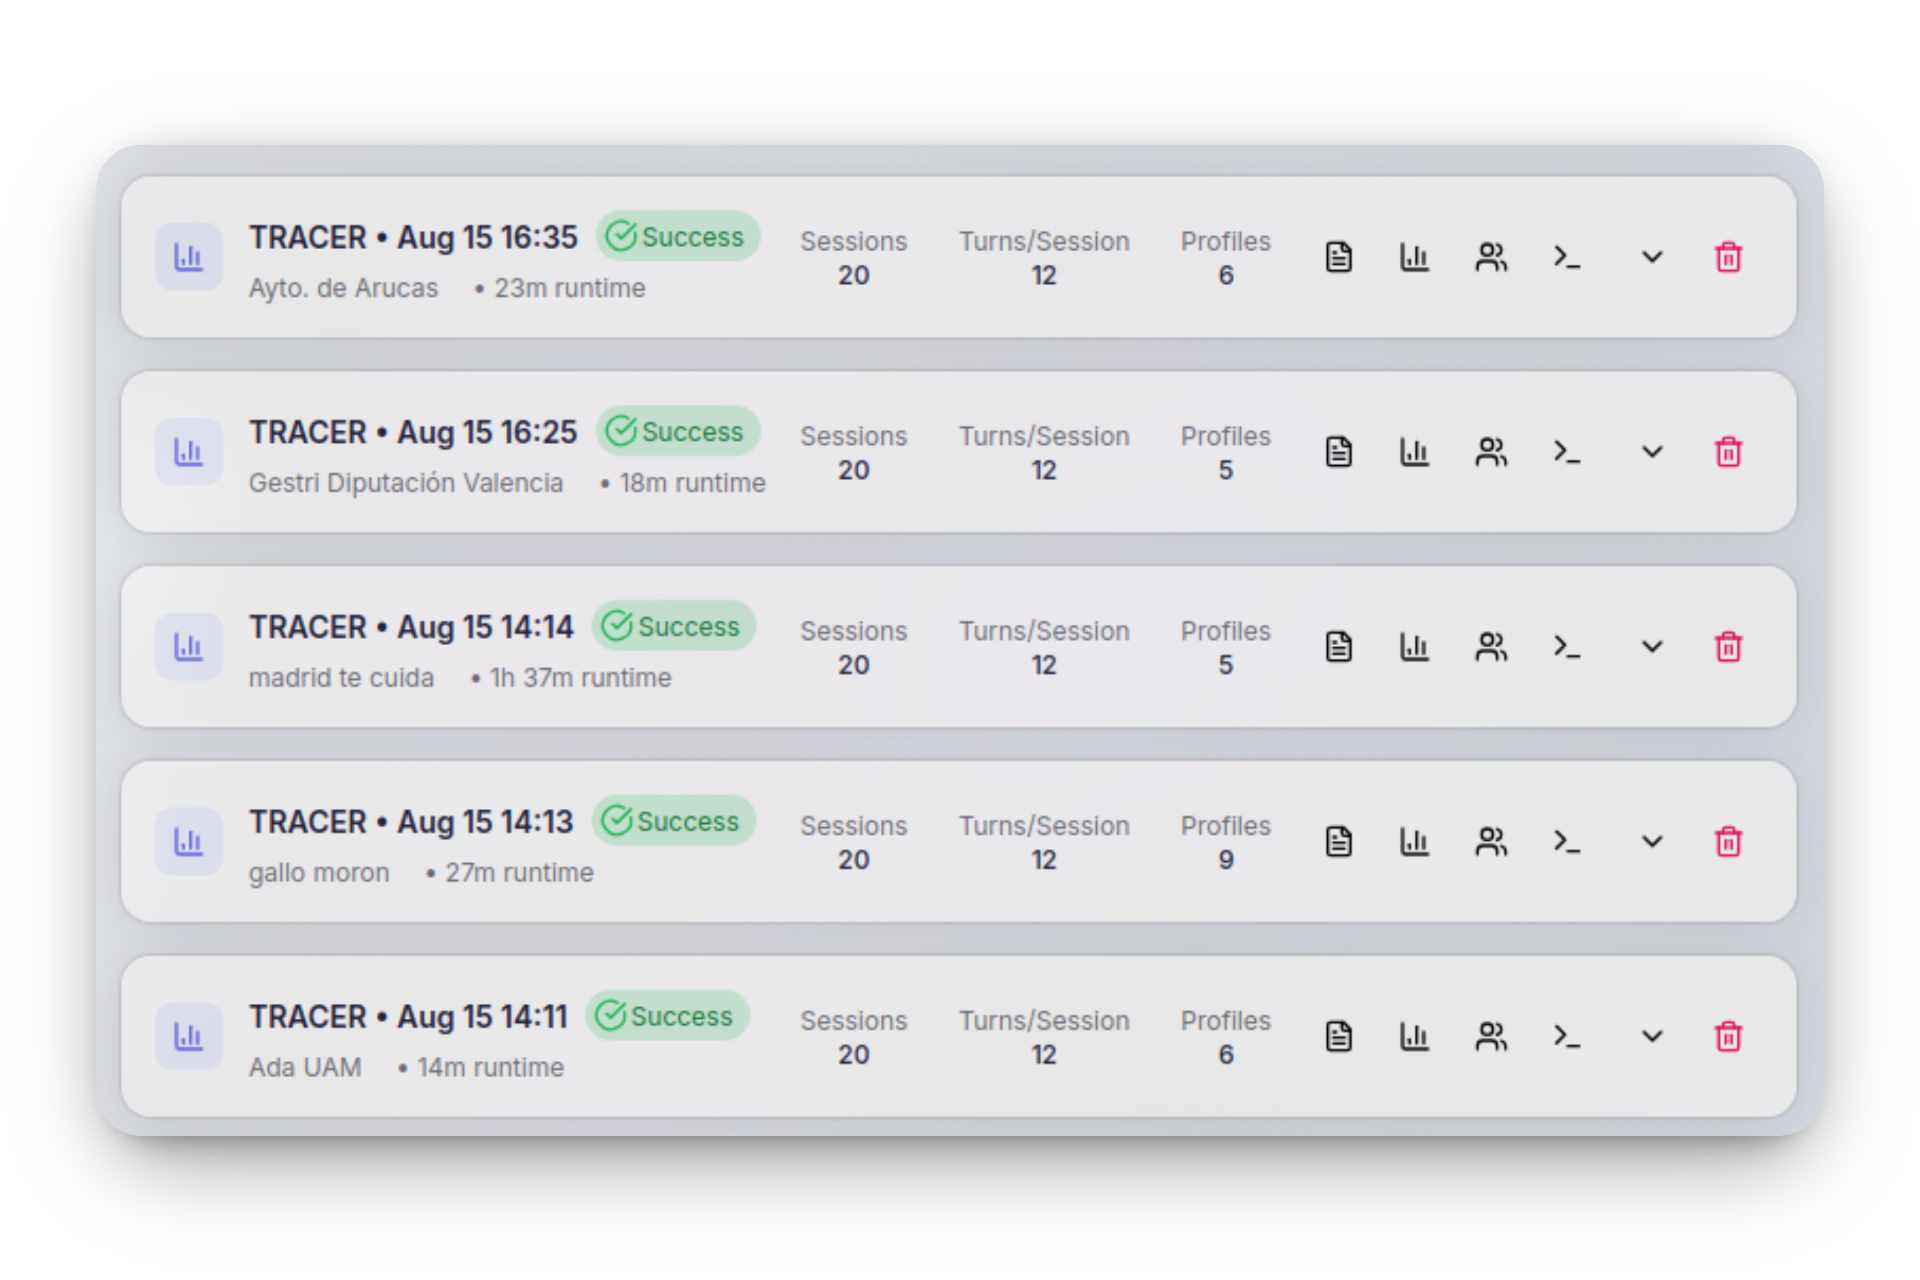
\includegraphics[width=\textwidth]{figures/tracer-results.png}
  \end{center}
  \caption{Screenshot of the web application showing
    the TRACER executions that contain the results of the experiment.}
  \label{fig:tracer-results}
\end{figure}

The inferred models by \ac{TRACER} can be found at
\url{http://miso.ii.uam.es:8081/tracer-dashboard}.
The screenshot in \autoref{fig:tracer-results}
shows the executions that contain the results of this experiment.
The projects are set to public
so that the results can be consulted
without needing to sign up on the web application.

\autoref{tab:rq3_precision_results}
summarizes the results of the manual verification for each of the five chatbots.
The table is divided into five columns; the first is the chatbot under testing.
\texttt{\# Func. (TRACER)} is the number of functionalities
found by \ac{TRACER}.
\texttt{\ac{TP}} is the number of those functionalities
that have been manually validated, i.e.,
the chatbot exhibits those functionalities
and are not duplicated.
Meanwhile, \texttt{\ac{FP}} represents those
that have been verified to be incorrect or duplicated.
Lastly, we have the \texttt{Precision} computed as shown in \autoref{eq:precision}.

\begin{table}[htpb]
\centering
\caption{Precision of TRACER's Inferred Models for Deployed Chatbots.}
\label{tab:rq3_precision_results}
\begin{tabular}{@{}lcccc@{}}
\toprule
\textbf{Chatbot} & \textbf{\thead{\# Func. \\ (TRACER)}} & \textbf{\thead{TP \\ (Verified)}} & \textbf{\thead{FP \\ (Incorrect/Duplicate)}} & \textbf{\thead{Precision (\%)}} \\ \midrule
Ada-UAM & 22 & 22 & 0 & 100.0 \\
Gallo de Morón & 29 & 27 & 2 & 93.1 \\
Madrid te Cuida & 91 & 88 & 3 & 96.7 \\
Gestri & 27 & 27 & 0 & 100.0 \\
Arucas & 41 & 37 & 4 & 90.2 \\ \midrule
\textbf{Total} & 210 & 201 & 9 & \textbf{96.0} \\ \bottomrule
\end{tabular}
\end{table}

An average precision of 96.0\% can be observed,
with a minimum of 90.2\% in the Arucas Town Hall chatbot.
A perfect score of a 100\% was achieved
on the simple chatbots Ada-UAM and Gestri.
And a 96.7\% was obtained in Madrid te Cuida,
the most complex chatbot tested with 91 discovered functionalities,
which 88 of them were verified to be valid and unique.

All but one of the \acp{FP} were duplicates.
This means that out of the 210 discovered functionalities,
only one was hallucinated,
i.e., 99.52\% of the functionalities
are real functionalities exhibited by the chatbot.
The hallucinated functionality was a claim that
Gallo de Morón offered a service to claim lottery prizes,
which it does not.
The remainder of the \acp{FP} were all duplicates
in which the LLM identified two very similar functionalities.
For example, in the 'Arucas' chatbot,
\ac{TRACER} created separate nodes for
'Present Electronic Office Options'
and 'Provide Electronic Office link'.
This indicates that while TRACER's discovery process is robust,
the automated consolidation logic can be further improved.

\subsection{Threats to Validity}

The primary threat to this experiment is
the inability to calculate the recall.
This is due to the nature of black-box systems,
which makes obtaining a ground-truth model of the chatbot infeasible.
Therefore, while the correctness of the inferred model (precision)
was effectively measured,
its completeness (recall)
could not be quantitatively assessed and remains an open question.

\subsection{Answer to RQ3}

The results of this experiment allow us to positively answer RQ3.
\ac{TRACER} demonstrated its ability
to accurately model the functionalities of
real-world, deployed chatbots, achieving an average precision of 96.0\%.
The qualitative analysis revealed that
the errors were not due to the hallucination of false functionalities
but rather to an over-granularity in distinguishing
between semantically similar features.
This confirms that \ac{TRACER} is a precise tool
to automatically model chatbots
in a black-box and real-world scenario.

